\section{Results}

Porta eget eu magnis luctus vestibulum ad interdum litora platea neque sed at felis urna velit, a fusce laoreet aptent sapien fringilla montes posuere facilisi iaculis orci libero penatibus nullam. Montes scelerisque quisque phasellus praesent per sed iaculis, porttitor proin penatibus varius luctus cras primis cubilia, fusce rhoncus vestibulum magnis vitae tincidunt. Dignissim mollis lacus pharetra semper lobortis id convallis natoque porta orci, magnis venenatis sodales erat metus integer vitae habitasse conubia, congue est enim dis interdum quisque egestas sociosqu aenean \footnote{ I prefer not to show all my attempts in this document but I have made a previous analysis and documentation
on a Jupyter Notebook that can be found at \url{https://github.com/ValentinaBustos2025/Proyecto-Final} in a Jupyter Notebook, in the file
\textbf{Simulación/Simulacion Principal.ipynb}.}. \\


\subsection{Constant-Payoff Evolutionary Regimes}



As mentioned in the methodology, the python \texttt{scipy.optimize} library was used to find the values of  \(\eta_d\)  and  \(r_0\)  giving summarized values in the table \ref{tab:linermatrixdynamics}.  To illustrate these regimes, figure \ref{fig:replicator} presents the evolutionary trajectories of the proportion of phenotype A, \(p(t)\), for representative combinations of \(\eta_d\) and \(r_0\), considering different initial population compositions. The boundary conditions \(p=0\), corresponding to a population composed entirely of phenotype B, and \(p=1\), corresponding to a population composed entirely of phenotype A, were excluded from the plotted initial conditions because both are stationary states of the replicator equation (\(\dot{p}=0\)), where the phenotypic composition remains unchanged. Therefore, only initial frequencies satisfying \(0<p(0)<1\) were considered to visualize the evolution of the population toward the corresponding equilibria. 

\begin{figure}[h!]
    \centering
    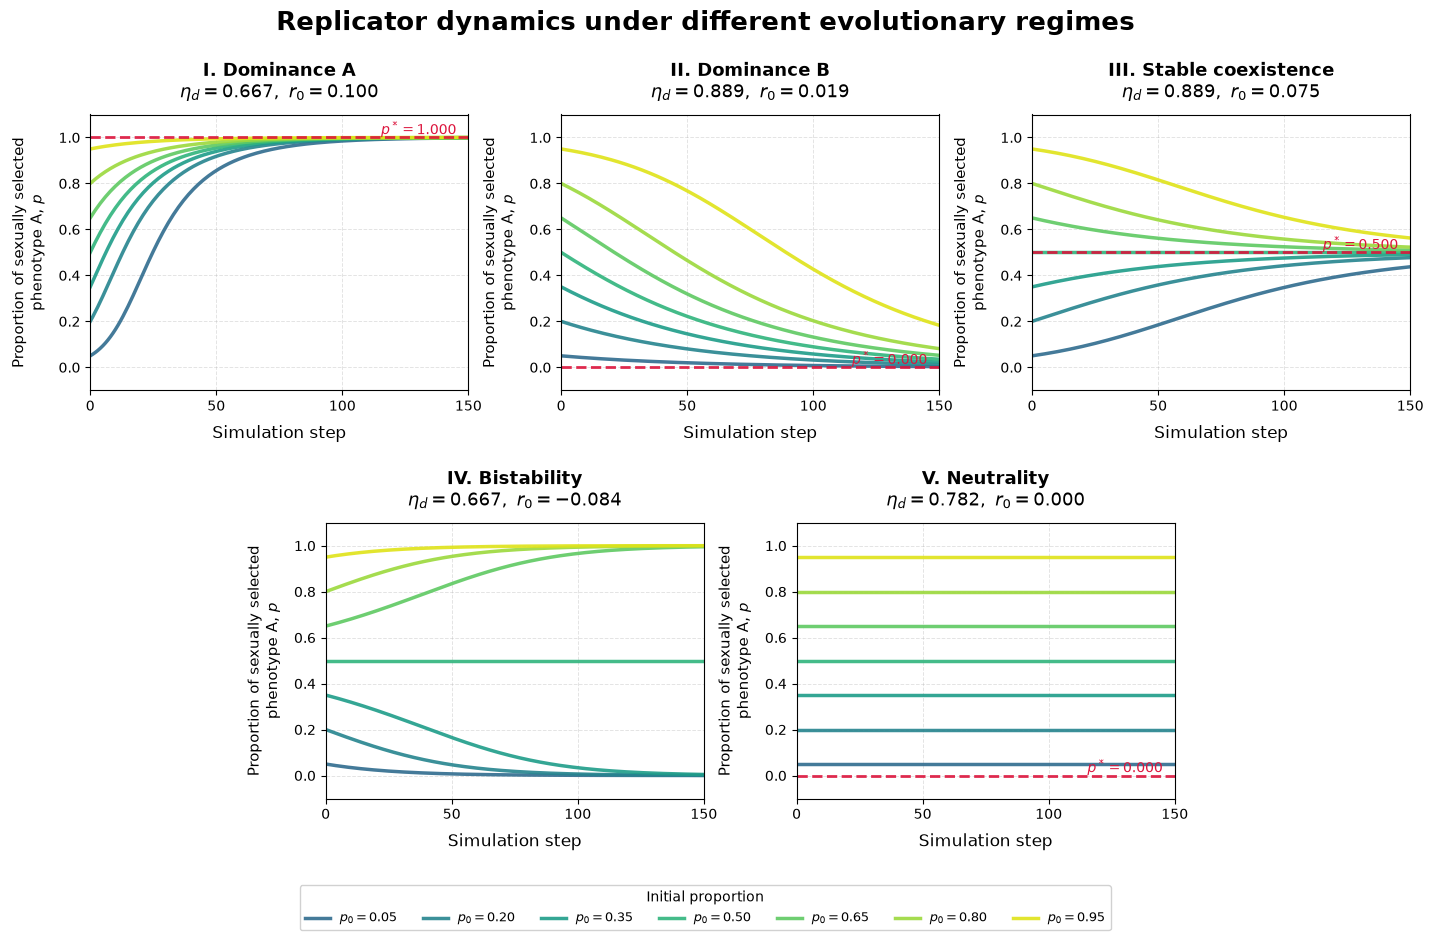
\includegraphics[width=1\linewidth]{Imagenes/Replicator.png}
    \caption{Deterministic replicator dynamics of the sexually selected phenotype A under five evolutionary regimes: (I) A dominance, (II) B dominance, (III) stable coexistence, (IV) bistability, and (V) neutrality. Each curve represents a different initial phenotype frequency ($p_0$), while predation intensity ($\eta_d$) and reproductive advantage ($r_0$) remain fixed within each scenario. The horizontal axis represents simulation steps in arbitrary time units, and the vertical axis represents the proportion of phenotype A. The corresponding frequencies maximizing mean population fitness are $p_{\max}\approx0.7105$, $0$, $0.25$, and $1$ for regimes I--IV, respectively. In the neutral regime (V), mean fitness is constant for all population compositions. These fitness maxima do not necessarily coincide with the stable evolutionary equilibria.}
    \label{fig:replicator}
\end{figure}



\begin{table}[!ht]
\centering
\caption{Evolutionary regimes obtained from the numerical
parameter search of the constant-payoff model. The parameters
$\eta_d$ and $r_0$ were determined using SciPy. A dominance,
B dominance, stable coexistence, and neutrality were identified,
whereas bistability was not found within the investigated
parameter range.}
\label{tab:linermatrixdynamics}

\begin{tabular}{l c c l c}
\toprule
Regime & $\eta_d$ & $r_0$ &
Equilibrium / stability & ESS \\
\midrule

A dominance
& $0.593052$ & $0.082638$
& $p^*=1$ (stable) & A \\

B dominance
& $0.937813$ & $0.026465$
& $p^*=0$ (stable) & B \\

Stable coexistence
& $0.870670$ & $0.244946$
& $p^*=0.873261$ (stable) & Mixed \\

Neutrality
& $0.781889$ & $\approx 0$
& All $p$ (neutral) & None \\

\bottomrule
\end{tabular}
\end{table}




\subsection{Frequency-Dependt  Evolutionary Equilibria}

We computationally analyzed the frequency-dependent replicator equation by sweeping predation intensity (\(\eta_d\)) and the initial proportion of phenotype A (\(p_0\)). This parameter sweep revealed two evolutionary regimes (table \ref{tab:frequencydependentdynamics}): A dominance and stable A-B coexistence. The figure \ref{fig:replicator} displays the deterministic trajectories for \(\eta_d = 0\) and \(\eta_d = 0.510\) across seven initial population compositions. Although the convergence paths differ, trajectories converge to the same equilibrium for a given \(\eta_d\), regardless of \(p_0\). However, this equilibrium frequency shifts with \(\eta_d\) (see \texttt{tabla\_dinamicas\_frecuencia.csv} in the notebook). We excluded the boundary conditions \(p=0\) and \(p=1\) (pure populations of B or A, respectively) because they are stationary states of the replicator equation (\(\dot{p}=0\)). Consequently, only initial proportions \(0 < p_0 < 1\) were plotted to illustrate convergence toward the evolutionary equilibria.\\ 


\begin{figure}[h!]
    \centering
    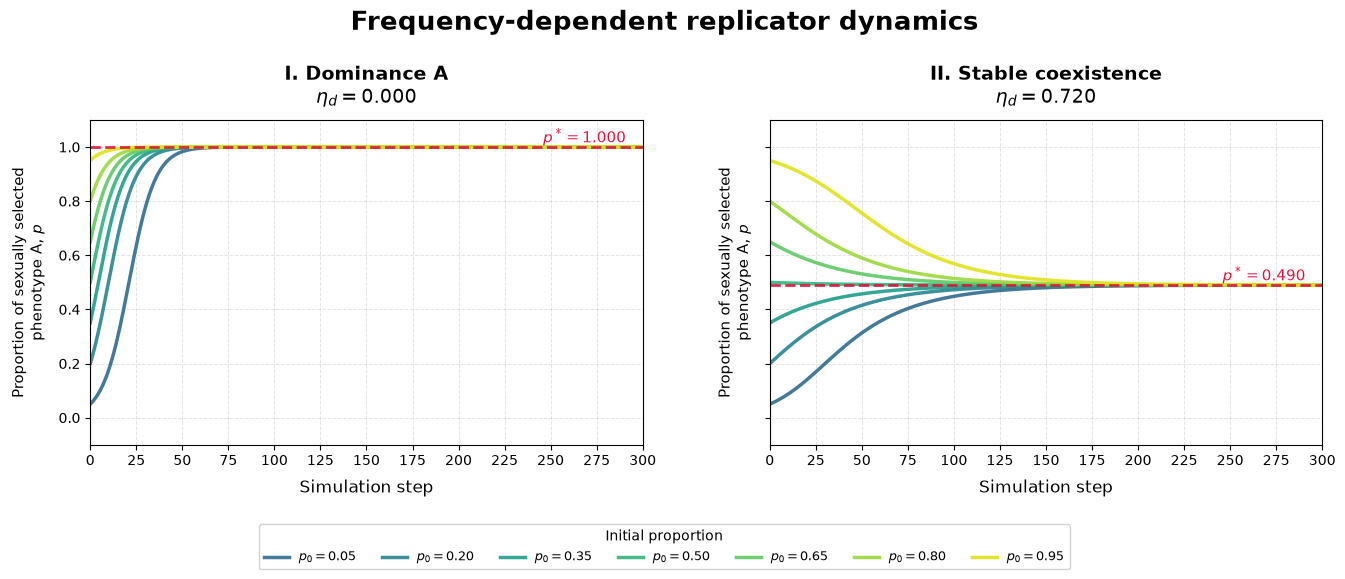
\includegraphics[width=1\linewidth]{Imagenes/ReplicatorFreqDep.png}
    \caption{ Deterministic replicator dynamics of the sexually selected phenotype A under two evolutionary regimes: (I) dominance of phenotype A at \((\eta_d=0)\) and (II) stable coexistence at \((\eta_d=1)\). Each curve represents a different initial proportion of phenotype A (\(p_0)\), while predation intensity \(\eta_d)\) remains fixed within each scenario. The horizontal axis represents simulation steps in arbitrary time units, whereas the vertical axis represents the proportion of phenotype A in the population, \(p\). In both regimes, trajectories with different initial proportions converge toward the same equilibrium, determined by the corresponding predation intensity.}
    \label{fig:replicatorFreqDep}
\end{figure}


\begin{table}[!ht]
\centering
\caption{Summary of the evolutionary regimes observed
in the frequency-dependent payoff model as a function
of predation intensity ($\eta_d$). The transition
between dominance of phenotype A and stable coexistence
occurs at approximately $\eta_d = 0.510$.}
\label{tab:frequencydependentdynamics}

\begin{tabular}{l c l c}
\toprule
Regime & $\eta_d$ & Stable equilibrium & ESS of A \\
\midrule
A dominance
& $0 \leq \eta_d < 0.510$
& $p^*=1$ & Yes \\

Stable coexistence
& $0.510 < \eta_d \leq 1$
& $0<p^*<1$ & No \\
\bottomrule
\end{tabular}
\end{table}

\clearpage 

\subsection{Stochastic Dynamics and Fixation}

\subsection{Effects of Nonlinear Sexual Saturation}

\subsection{Comparasion of Evolutionary Models}


\section{Discussion}

Porta eget eu magnis luctus vestibulum ad interdum litora platea neque sed at felis urna velit, a fusce laoreet aptent sapien fringilla montes posuere facilisi iaculis orci libero penatibus nullam. Montes scelerisque quisque phasellus praesent per sed iaculis, porttitor proin penatibus varius luctus cras primis cubilia, fusce rhoncus vestibulum magnis vitae tincidunt. Dignissim mollis lacus pharetra semper lobortis id convallis natoque porta orci, magnis venenatis sodales erat metus integer vitae habitasse conubia, congue est enim dis interdum quisque egestas sociosqu aenean. \\ 





Primero, la dependencia de la frecuencia. Compararías si introducir una vulnerabilidad que cambia con la composición del cardumen modifica las condiciones de coexistencia respecto al modelo de pagos constantes. Aquí puedes hablar de los mecanismos biológicos, incluidos oddity y confusion, sin afirmar que tus funciones representan exactamente todos esos efectos.\\ 

Segundo, la diferencia entre coexistencia determinista y persistencia estocástica. Esta sería posiblemente la comparación más potente desde la física estadística: la existencia de un equilibrio estable no garantiza la permanencia de ambos fenotipos en una población finita sin mutaciones.

Tercero, la saturación sexual. Discutirías si una ventaja reproductiva que disminuye con la abundancia de machos atractivos puede contrarrestar o reforzar los efectos de la depredación. Aquí sería importante aclarar qué parte de esa función es una hipótesis fenomenológica y qué parte está motivada por evidencia biológica. 

\subsection{Linear Payoff Matrix }
The constant-payoff model provides a deterministic reference for examining the competition between sexual selection and predation. As shown in table \ref{tab:linermatrixdynamics} and figure \ref{fig:replicator}, three main evolutionary regimes emerge: dominance of phenotype A, dominance of phenotype B, and stable coexistence. Phenotype A is favored at lower predation intensities, whereas stronger predation may favor phenotype B unless the reproductive advantage \(r_0\) is sufficient to maintain an interior equilibrium. Two additional cases were examined: bistability, in which the evolutionary outcome depends on the initial population composition, and neutrality, where the fitness difference vanishes and all population compositions remain stationary. However, bistability requires \(r_0<0\), representing a reproductive disadvantage for phenotype A and therefore falling outside the biologically motivated parameter range. It is consequently retained as a mathematical extension, while neutrality represents a limiting case in which neither phenotype has a selective advantage. \\ 



 *Se incluyó inicilamente el metodo Wright- Fisher como un método de comparación. Se vio muy claramente que no era muy realista y que no se ajustaba a la realidad de la población de peces guppy. Por lo tanto, se decidió no incluirlo en el análisis final.\\
